\ifx\mainfile\undefined
%  ========================================================================
%  Copyright (c) 2006-2011 The University of Washington
%
%  Licensed under the Apache License, Version 2.0 (the "License");
%  you may not use this file except in compliance with the License.
%  You may obtain a copy of the License at
%
%      http://www.apache.org/licenses/LICENSE-2.0
%
%  Unless required by applicable law or agreed to in writing, software
%  distributed under the License is distributed on an "AS IS" BASIS,
%  WITHOUT WARRANTIES OR CONDITIONS OF ANY KIND, either express or implied.
%  See the License for the specific language governing permissions and
%  limitations under the License.
%  ========================================================================
%
 
\documentclass [11pt, twoside] {uwthesis}

\usepackage{color}
\usepackage{url}
\usepackage{amsmath}
\usepackage{amsfonts}
\usepackage[bookmarks,
	hidelinks,
	plainpages=false,
	pdfpagelabels,
	pagebackref=true,
            ]{hyperref}
\renewcommand*{\backref}[1]{}% for backref < 1.33 necessary
\renewcommand*{\backrefalt}[4]{%
  \ifcase #1 %
    (No citations.)%
  \or
    (Cited on page #2.)%
  \else
    (Cited on pages #2.)%
  \fi
}

\newcommand{\biburl}[1]{{\tt<}\url{#1}{\tt>}}

\hypersetup{%
pdfauthor = {Daniel Chaim Halperin},
pdftitle = {Simplifying the Configuration of 802.11 Wireless Networks with Effective SNR},
pdfsubject = {Ph.D. Dissertation},
pdfkeywords = {},
pdfcreator = {University of Washington, Computer Science and Engineering},
pdfproducer = {},
bookmarksopen = {true},
pdfpagelayout = {TwoColumnRight},
}

\usepackage{footnotebackref}
%%%%%%%%%%%%%%%%%%%%%%%%%%%%%%%%%%%%%%%%%%%%%%%%%%%%%%
%%%        Formatting sections                     %%%
%%%%%%%%%%%%%%%%%%%%%%%%%%%%%%%%%%%%%%%%%%%%%%%%%%%%%%
\newcommand{\algref}[1]{Algorithm~\ref{#1}}
\newcommand{\chapref}[1]{Chapter~\ref{#1}}
\renewcommand{\eqref}[1]{Equation~\ref{#1}}
\newcommand{\figref}[1]{Figure~\ref{#1}}
\newcommand{\secref}[1]{\S\ref{#1}}
\newcommand{\tabref}[1]{Table~\ref{#1}}
\newcommand{\heading}[1]{\vspace{4pt}\noindent\textbf{#1}}
\newcommand{\topheading}[1]{\noindent\textbf{#1}}
\newcommand{\noheading}[0]{\vspace{4pt}\noindent}

%%%%%%%%%%%%%%%%%%%%%%%%%%%%%%%%%%%%%%%%%%%%%%%%%%%%%%
%%%        XXX and other warnings                  %%%
%%%%%%%%%%%%%%%%%%%%%%%%%%%%%%%%%%%%%%%%%%%%%%%%%%%%%%
\newcommand{\xxx}[1]{\textit{\color{red}XXX #1}}

%%%%%%%%%%%%%%%%%%%%%%%%%%%%%%%%%%%%%%%%%%%%%%%%%%%%%%
%%%        Units                                   %%%
%%%%%%%%%%%%%%%%%%%%%%%%%%%%%%%%%%%%%%%%%%%%%%%%%%%%%%
\usepackage{xspace}
\newcommand{\unitsep}{\texorpdfstring{\,}{ }}
\def\unit#1{% from: http://www.tex.ac.uk/cgi-bin/texfaq2html?label=csname "Defining a macro from an argument"
  \expandafter\def\csname #1\endcsname{\unitsep\text{#1}\xspace}%
}
\def\varunit#1#2{% from: http://www.tex.ac.uk/cgi-bin/texfaq2html?label=csname "Defining a macro from an argument"
  \expandafter\def\csname #1\endcsname{\unitsep\text{#2}\xspace}%
}
\unit{GHz}
\unit{MHz}
\unit{kHz}
\unit{Gbps}
\unit{Mbps}
\unit{KB}
\unit{dB}
\unit{dBi}
\unit{dBm}
\unit{W}
\unit{mW}
\varunit{uW}{$\mu$W}
\unit{ms}
\varunit{us}{$\mu$s}
\unit{h}
\unit{m}
\unit{s}
\unit{km}
\unit{cm}
\unit{mm}
\varunit{mmsq}{mm$^\text{2}$}
\varunit{insq}{in$^\text{2}$}
\newcommand{\degree}{\ensuremath{^\circ}\xspace}
\newcommand{\degrees}{\degree}
%%%%%%%%%%%%%%%%%%%%%%%%%%%%%%%%%%%%%%%%%%%%%%%%%%%%%%%%%%%%%%%%%%%%%%%%%%%%%%%%%%%%%%
% Euler for math | Palatino for rm | Helvetica for ss | Courier for tt
%
% From: http://www.tug.org/mactex/fonts/LaTeX_Preamble-Font_Choices.html
%%%%%%%%%%%%%%%%%%%%%%%%%%%%%%%%%%%%%%%%%%%%%%%%%%%%%%%%%%%%%%%%%%%%%%%%%%%%%%%%%%%%%%
\renewcommand{\rmdefault}{ppl} % rm
\usepackage[scaled]{helvet} % ss
\usepackage{courier} % tt
\usepackage{eulervm} % a better implementation of the euler package (not in gwTeX)
\normalfont
\usepackage[T1]{fontenc}
%%%%%%%%%%%%%%%%%%%%%%%%%%%%%%%%%%%%%%%%%%%%%%%%%%%%%%%%%%%%%%%%%%%%%%%%%%%%%%%%%%%%%%

%%%%%%%%%%%%%%%%%%%%%%%%%%%%%%%%%%%%%%%%%%%%%%%%%%%%%%
%%%        Figures                                 %%%
%%%%%%%%%%%%%%%%%%%%%%%%%%%%%%%%%%%%%%%%%%%%%%%%%%%%%%
\usepackage{graphicx}
% Caption package both lets you set the spacing between figure and caption
% and also makes the \figref{} point to the right place.
\usepackage[font=bf,aboveskip=6pt,belowskip=-4mm]{caption}
% Allow subfigures, make them bold
\usepackage[bf,BF,small]{subfigure}
% List of figures
\setcounter{lofdepth}{2}  % Print the chapter and sections to the lot

%%%%%%%%%%%%%%%%%%%%%%%%%%%%%%%%%%%%%%%%%%%%%%%%%%%%%%
%%%        Lists with reduced spacing              %%%
%%%%%%%%%%%%%%%%%%%%%%%%%%%%%%%%%%%%%%%%%%%%%%%%%%%%%%
\usepackage{enumitem}

%%%%%%%%%%%%%%%%%%%%%%%%%%%%%%%%%%%%%%%%%%%%%%%%%%%%%%
%%%        Fancy tables                            %%%
%%%%%%%%%%%%%%%%%%%%%%%%%%%%%%%%%%%%%%%%%%%%%%%%%%%%%%
\usepackage{tabulary}
\usepackage{booktabs}

%%%%%%%%%%%%%%%%%%%%%%%%%%%%%%%%%%%%%%%%%%%%%%%%%%%%%%
%%%        Formatting techniques/tools/etc.        %%%
%%%%%%%%%%%%%%%%%%%%%%%%%%%%%%%%%%%%%%%%%%%%%%%%%%%%%%
\newcommand{\term}[1]{\texttt{#1}}

\begin{document}
 
\textpages
\setcounter{chapter}{4} % Set to n-1!
\fi
%%%%%%%%%%%%%%%%%%%%%%%%%%%%%%%%%%

\cleardoublepage
\chapter{Experimental Setup}
\label{chap:tool}

In this chapter, I describe my experimental 802.11n platform, which comprises a prototype implementation of a CSI measurement tool based on commodity Intel Wi-Fi NICs and experimental 802.11n wireless testbeds in two indoor office environments. I also describe the comprehensive datasets on which I base my experiments. This experimental setup is the foundation of the experimental results in the remainder of my thesis.

\section{802.11n CSI Tool and Experimental Platform}
\label{sec:platform}
In conjunction with Intel Labs Seattle, I built an experimental 802.11n platform that uses the Intel Wi-Fi Wireless Link 5300 (IWL5300) 802.11a/b/g/n network cards (\figref{fig:iwl5300}). These 802.11n MIMO NICs have three antennas and support many new features of 802.11n. I modified the closed-source firmware and open-source \program{iwlwifi} driver for Linux to add a number of experimental features and, crucially, to measure the 802.11n CSI.

\begin{figure}
	\centering
	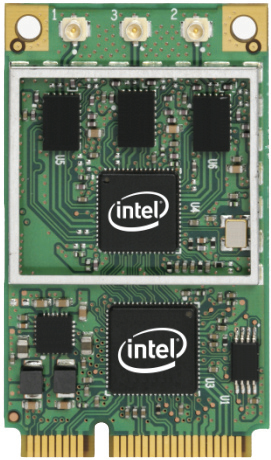
\includegraphics[height=2in]{figures/iwlwifi-5300.png}
	\caption[The Intel Wireless Wi-Fi Link 5300]{\label{fig:iwl5300}The Intel Wireless Wi-Fi Link 5300. This 802.11n NIC has three transmit/receive antennas, operates on both 2.4\GHz and 5\GHz frequency bands, and supports up to three spatial streams for a maximum bitrate of 450\Mbps.}
\end{figure}

\heading{802.11n CSI Measurement.} The channel sounding mechanism added in 802.11n defines a management frame used to report the CSI from the receiver of a frame back to the transmitter. This mechanism is intended for calibration or to inform transmit beamforming, and I co-opt it for my experiments. In standard operation, the CSI is reported only when the sounding procedure is initiated by the transmitter, though the receiver measures CSI for every frame in order to receive the packet. In my tool, I configure the NIC with a debug mode to compute this feedback packet for every received frame, rather than just during sounding. For correctly received packets, the firmware will send it up to the driver on the receiving node.

The IWL5300 provides CSI in a format that reports the channel matrices for 30 subcarrier groups, which is about one group for every 2 subcarriers at 20\MHz or every 4 subcarriers at 40\MHz. Each channel matrix entry is a complex number, with signed 8-bit resolution each for the real and imaginary parts. It specifies the gain and phase of the spatial path between a single transmit-receive antenna pair. Intel's implementation of the 802.11n CSI does not include per-subcarrier noise measurements, so I assume the noise floor is uniform across all subcarriers to compute SNRs. This is consistent with white noise observed on other OFDM platforms~\cite{Rahul_FARA}.

\heading{RSSI Measurement.} 
For each received packet the NIC reports the traditional metrics of RSSI per receive antenna, noise floor and the setting on the automatic gain controlled (AGC) amplifier. These combine to define the per-receive-chain Packet SNR ($\rho_{\text{packet}}$):
\begin{equation}
\label{eq:per_chain_snr}
	\rho_{\text{packet}} = \text{RSSI (dBm)} - \text{Noise (dBm)} - \text{AGC (dB)}
\end{equation}
The IWL5300 calculates the quantities RSSI and Noise as the respective sums of average signal strength and average error vector magnitude in each OFDM subcarrier~\cite{iwlwifi}. This is exactly the traditional definition of SNR applied to OFDM.

\heading{Transmit Power Control.} I modified the driver and firmware to enable transmit power variation. With these changes, I can vary the transmit power level from $-$10\dBm~(100\uW) to $+$16\dBm~(40\mW) in steps of 0.5\dB. For all modulations, the IWL5300 divides power equally across transmit antennas. Additionally, the IWL5300 reduces the transmit power slightly when using the highest single-stream rates to avoid distortions caused by passing 64-QAM symbols with high peak-to-average power ratio through the transmit amplifier.

\heading{Rapid Rate Variation.} In normal operation, the IWL5300 decouples queuing packets for transmission from selecting rates for these packets, since queues must be kept large to take advantage of 802.11n block transmissions. This makes it difficult to control the rate at which individual packets are transmitted. I modified the firmware and driver to support the transmission of individual packets at predetermined rates, and added driver-level code to rapidly iterate through a user-configurable set of available rates.

\heading{Userspace Connector.} I used the Linux kernel \program{connector} framework to implement a low-latency socket-based communication channel between the kernel driver and userspace utilities. This enables userspace utilities to log CSI and other output from the driver, and send messages that adapt behavior online, e.g., by changing the currently selected rate or antennas or adjusting the transmit power level.

\heading{Publicly Released Tool.} I have publicly released the experimental platform and CSI collection tool in the form of open source drivers, userspace utilities, MATLAB data processing code, and binary firmware image~\cite{Halperin_csitool}. At the time of writing, I am aware of 17 universities in 7 countries, multiple research and product groups within Intel, one industrial research labs and one startup using my tool. The users of my tool have published at least 5 papers~\cite{Bhartia_FreqDiv,Crepaldi_CSI_SF,Perahia_Doppler,Sen_SpinLoc,Sen_PinLoc}.

%%%%%%%%%%%%%%%%%%%%%%%%%%%%%%%%%%
\section{Experimental 802.11n Wireless Testbeds}
I conducted experiments in two 802.11n stationary wireless testbeds. The first testbed, pictured in \figref{fig:intel_testbed}, contains 10 nodes spread over one floor of Intel Labs Seattle covering 8,100 square feet. In the second testbed, I deployed 24 nodes across 3 floors in UW CSE (\figref{fig:uw_testbed}), where each floor measures approximately 20,000 square feet in size. Both testbeds are indoor office buildings, the former mostly a wide open area with cubicles and a few conference rooms, the latter consisting primarily of 5-person offices.

\begin{figure}[p]
	\centering
	\subfigure[The testbed at Intel Labs Seattle][The testbed at Intel Labs Seattle contained of 10 nodes spread over 8,100 square feet.\label{fig:intel_testbed}]{
		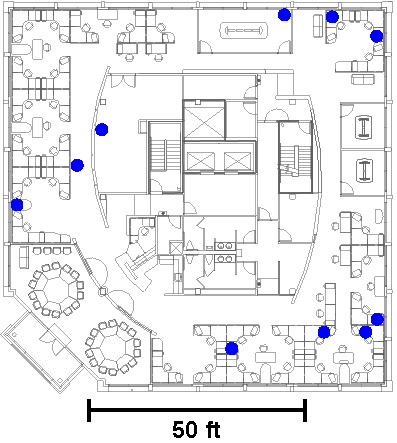
\includegraphics[scale=1.054]{figures/intel_floorplan_testbed.pdf}
    }
	\subfigure[The testbed at UW CSE][The testbed at the UW CSE comprises 24 nodes spread over 3 floors of 20,000 square feet.\label{fig:uw_testbed}]{
		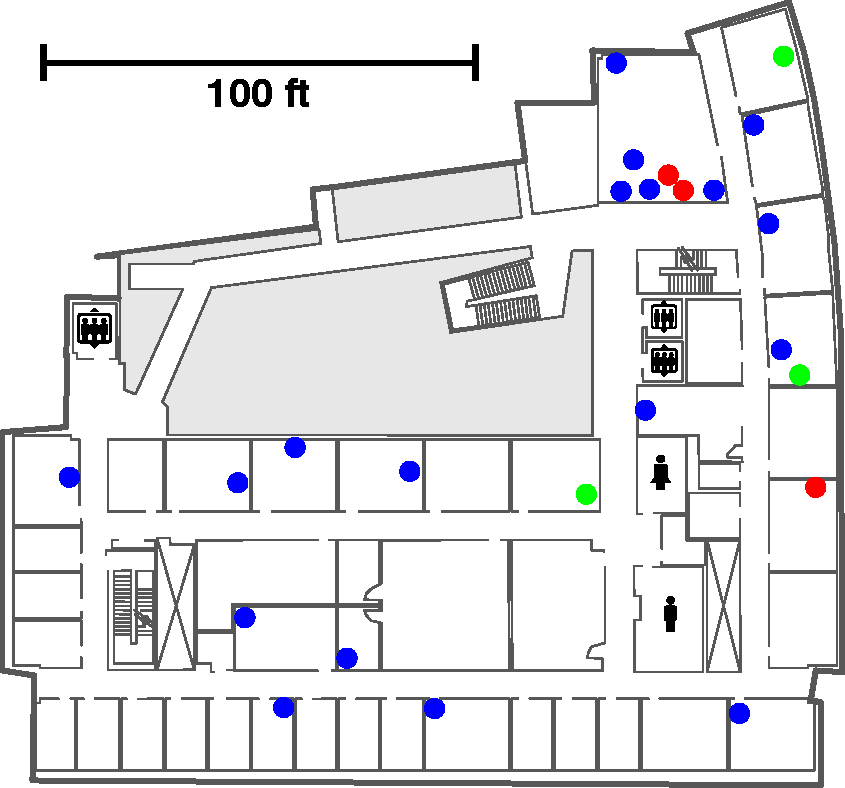
\includegraphics[scale=0.62]{figures/floor3_grayscale_noee_testbed.pdf}
	}
	\caption[My two indoor 802.11n testbeds]{\label{fig:testbeds} My two indoor 802.11n testbeds. In both testbeds, the nodes are placed to ensure a large number of links between them, a variety of distances between nodes, and diverse scattering characteristics.}
\end{figure}

Each node runs the experimental platform we described in \secref{sec:platform}, as do three laptops we can use for mobile experiments. In both testbeds, I placed the nodes to ensure a large number of links between them, a variety of distances between nodes, and diverse scattering characteristics. Devices are located on in a desktops, under tables, on a carts in the server room, and even mounted on the ceiling; in the UW CSE testbed also includes a more dense concentration of nodes by the Networking Lab (pictured in the upper right corner of \figref{fig:uw_testbed}).

\begin{figure}[ht]
	\centering
	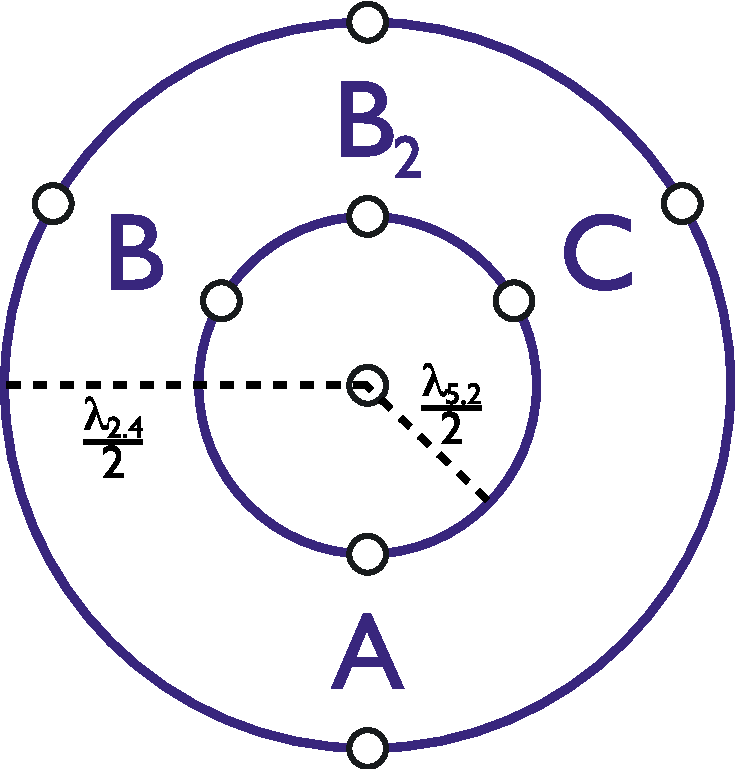
\includegraphics[width=1.5in]{figures/rpsma_dual_632_single_lines.pdf}%
	\hspace{1in}
	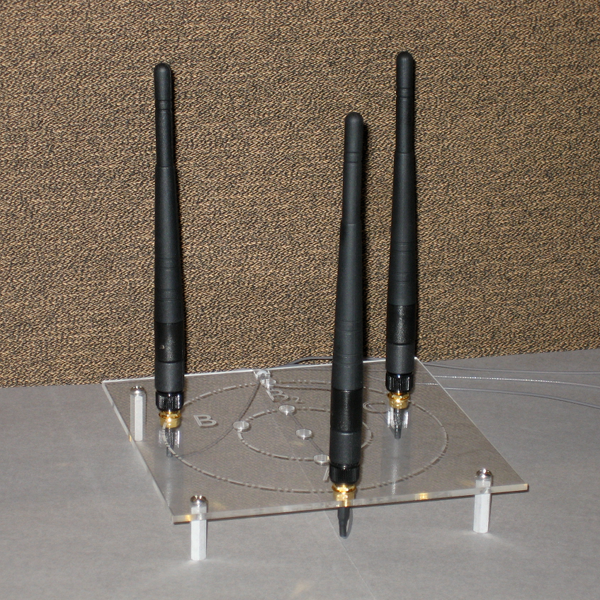
\includegraphics[height=1.5in,width=1.5in]{figures/antennas.png}
	\caption[A custom antenna stand used to achieve consistent spatial geometry]{\label{fig:antenna_stand}The antenna stand I use to achieve consistent spatial geometry for desktop machines. It supports circular and linear arrays of two or three antennas with the correct $\lambda/2$ separation at either 2.4\GHz or 5\GHz.}
\end{figure}
\begin{figure}[ht]
	\centering
	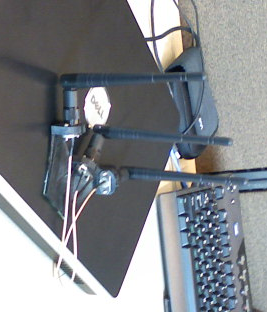
\includegraphics[angle=90,height=1.8in]{figures/laptop_stand_cropped_up.png}%
	\hspace{0.6in}%
	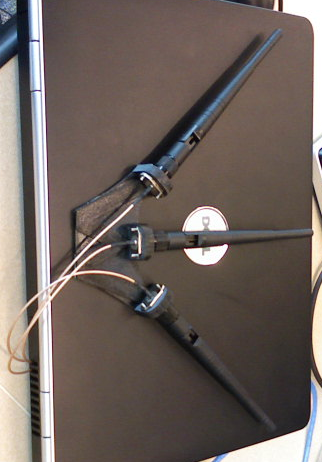
\includegraphics[angle=90,height=1.8in]{figures/laptop_stand_cropped.png}
	\caption[A custom laptop antenna stand]{\label{fig:laptop_stands}One of the three laptops, pictured here, includes a custom antenna mount for a 2.4\GHz linear array.}
\end{figure}

\section{Node Configuration}
Each node is a stationary desktop (\figref{fig:antenna_stand}) or portable laptop (\figref{fig:laptop_stands}) equipped with an IWL5300. As the antenna geometry is important for spatial diversity, I mount the three antennas per node on custom stands. Each antenna achieves 5\dBi gain for the 2.4\GHz band, and 3\dBi for the 5\GHz band.

The desktop stands (\figref{fig:antenna_stand}) allow for a circular array (using ports ABC) or a linear array of two or three (AB$_2$ and optionally center) antennas, with antenna separations of half the wavelength for either 2.4\GHz Channel 6 ($\lambda/2 = 6.15\cm$) or 5\GHz Channel 48 ($\lambda/2=2.86\cm$). In desktop experiments in this paper, I use the circular three-antenna configuration for the 2.4\GHz band. It is robust and suited to dual-band NICs that need the wider 2.4\GHz antenna separation. 

The three laptops use three different antenna configurations. One laptop has all three antennas embedded internally like in a commercial laptop deployment; one laptop uses the same antenna stand as the desktop machines to mimic their behavior in portable experiments. The third laptop, pictured in \figref{fig:laptop_stands}, includes a custom antenna mount for a 2.4\GHz linear array.
%%%%%%%%%%%%%%%%%%%%%%%%%%%%%%%%%%
\section{Datasets}
\textcolor{red}{add text here as I pass through the next few sections}

%%%%%%%%%%%%%%%%%%%%%%%%%%%%%%%%%%
\ifx\mainfile\undefined
%
% ==========   Bibliography   ==========
%
%\nocite{*}   % include everything in the uwthesis.bib file
\bibliographystyle{plain}
\bibliography{dhalperi_thesis}

\end{document}
\fi